\documentclass[10pt]{article}
\usepackage[polish]{babel}
\usepackage[utf8]{inputenc}
\usepackage[T1]{fontenc}
\usepackage{graphicx}
\usepackage[export]{adjustbox}
\graphicspath{ {./images/} }
\usepackage{amsmath}
\usepackage{amsfonts}
\usepackage{amssymb}
\usepackage[version=4]{mhchem}
\usepackage{stmaryrd}
\usepackage{multirow}

\title{EGZAMIN MATURALNY \\
 Z MATEMATYKI }

\author{}
\date{}


\begin{document}
\maketitle

\includegraphics[max width=\textwidth, center]{2024_11_21_dcf819de2d2eef051a0dg-01(1)}\\

\includegraphics[max width=\textwidth, center]{2024_11_21_dcf819de2d2eef051a0dg-01}

\section*{POZIOM PODSTAWOWY}
MAJ 2012

\begin{enumerate}
  \item Sprawdź, czy arkusz egzaminacyjny zawiera 18 stron (zadania 1-34). Ewentualny brak zgłoś przewodniczącemu zespołu nadzorującego egzamin.
  \item Rozwiązania zadań i odpowiedzi wpisuj w miejscu na to przeznaczonym.
  \item Odpowiedzi do zadań zamkniętych (1-25) przenieś na kartę odpowiedzi, zaznaczając je w części karty przeznaczonej dla zdającego. Zamaluj \(\square\) pola do tego przeznaczone. Błędne zaznaczenie otocz kółkiem i zaznacz właściwe.
  \item Pamiętaj, że pominięcie argumentacji lub istotnych obliczeń w rozwiązaniu zadania otwartego (26-34) może spowodować, że za to rozwiązanie nie będziesz mógł
\end{enumerate}

Czas pracy: 170 minut\\
dostać pełnej liczby punktów.\\
5. Pisz czytelnie i używaj tylko długopisu lub pióra z czarnym tuszem lub atramentem.\\
6. Nie używaj korektora, a błędne zapisy wyraźnie przekreśl.\\
7. Pamiętaj, że zapisy w brudnopisie nie będą oceniane.\\
8. Możesz korzystać z zestawu wzorów matematycznych, cyrkla i linijki oraz kalkulatora.\\
9. Na tej stronie oraz na karcie odpowiedzi wpisz swój numer PESEL i przyklej naklejkę z kodem.\\
10. Nie wpisuj żadnych znaków w części przeznaczonej dla egzaminatora.

\section*{Liczba punktów}
do uzyskania: 50

MMA-P1\_1P-122

\section*{ZADANIA ZAMKNIĘTE}
W zadaniach od 1. do 25. wybierz izaznacz na karcie odpowiedzi poprawnq odpowiedź.

\section*{Zadanie 1. (1 pkt)}
Cenę nart obniżono o \(20 \%\), a po miesiącu nową cenę obniżono o dalsze \(30 \%\). W wyniku obu obniżek cena nart zmniejszyła się o\\
A. \(44 \%\)\\
B. \(50 \%\)\\
C. \(56 \%\)\\
D. \(60 \%\)

\section*{Zadanie 2. (1 pkt)}
Liczba \(\sqrt[3]{(-8)^{-1}} \cdot 16^{\frac{3}{4}}\) jest równa\\
A. -8\\
B. -4\\
C. 2\\
D. 4

\section*{Zadanie 3. (1 pkt)}
Liczba \((3-\sqrt{2})^{2}+4(2-\sqrt{2})\) jest równa\\
A. \(19-10 \sqrt{2}\)\\
B. \(17-4 \sqrt{2}\)\\
C. \(15+14 \sqrt{2}\)\\
D. \(19+6 \sqrt{2}\)

Zadanie 4. (1 pkt)\\
Iloczyn \(2 \cdot \log _{\frac{1}{3}} 9\) jest równy\\
A. -6\\
B. -4\\
C. -1\\
D. 1

\section*{Zadanie 5. (1 pkt)}
Wskaż liczbę, która spełnia równanie \(|3 x+1|=4 x\).\\
A. \(x=-1\)\\
B. \(x=1\)\\
C. \(x=2\)\\
D. \(x=-2\)

\section*{Zadanie 6. (1 pkt)}
Liczby \(x_{1}, x_{2}\) są różnymi rozwiązaniami równania \(2 x^{2}+3 x-7=0\). Suma \(x_{1}+x_{2}\) jest równa\\
A. \(-\frac{7}{2}\)\\
B. \(-\frac{7}{4}\)\\
C. \(-\frac{3}{2}\)\\
D. \(-\frac{3}{4}\)

\section*{Zadanie 7. (1 pkt)}
Miejscami zerowymi funkcji kwadratowej \(y=-3(x-7)(x+2)\) sa\\
A. \(x=7, x=-2\)\\
B. \(x=-7, x=-2\)\\
C. \(x=7, x=2\)\\
D. \(x=-7, x=2\)

\section*{Zadanie 8. (1 pkt)}
Funkcja liniowa \(f\) jest określona wzorem \(f(x)=a x+6\), gdzie \(a>0\). Wówczas spełniony jest warunek\\
A. \(f(1)>1\)\\
B. \(f(2)=2\)\\
C. \(f(3)<3\)\\
D. \(f(4)=4\)

\section*{BRUDNOPIS}
\begin{center}

\includegraphics[max width=\textwidth]{2024_11_21_dcf819de2d2eef051a0dg-03}
\end{center}

\section*{Zadanie 9. (1 pkt)}
Wskaż wykres funkcji, która w przedziale \(\langle-4,4\rangle\) ma dokładnie jedno miejsce zerowe.\\
A.\\
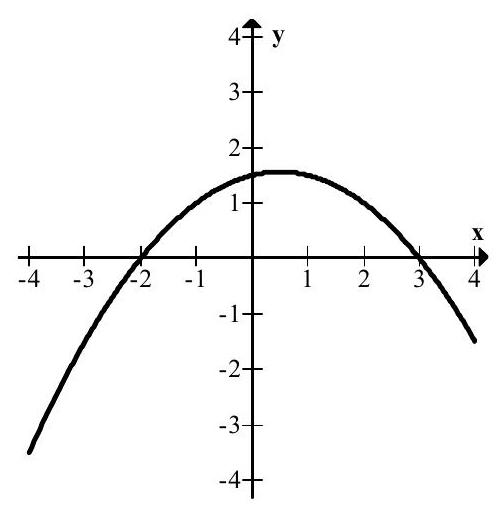
\includegraphics[max width=\textwidth, center]{2024_11_21_dcf819de2d2eef051a0dg-04}\\
C.\\
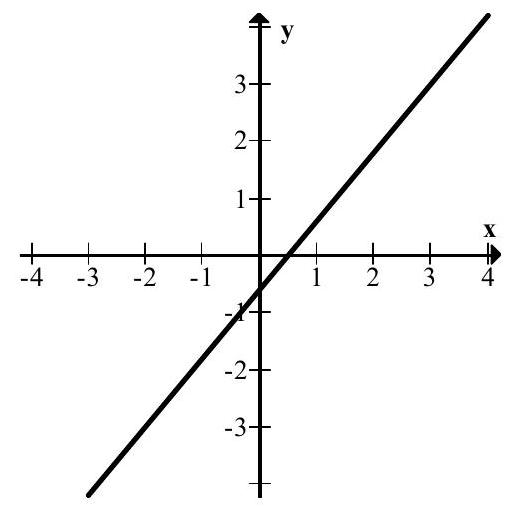
\includegraphics[max width=\textwidth, center]{2024_11_21_dcf819de2d2eef051a0dg-04(1)}\\
B.\\
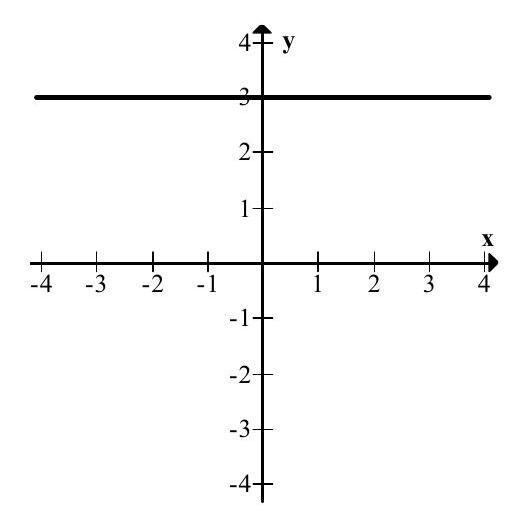
\includegraphics[max width=\textwidth, center]{2024_11_21_dcf819de2d2eef051a0dg-04(2)}\\
D.\\
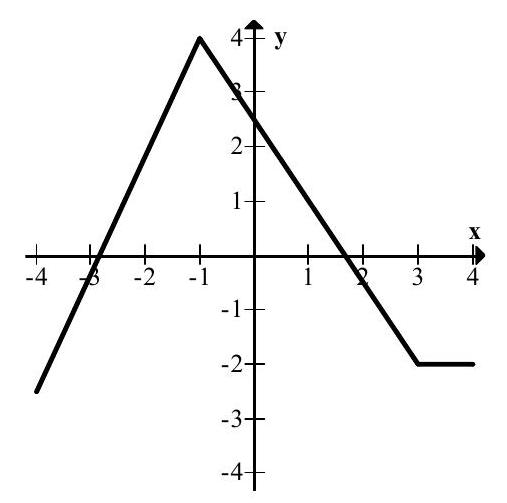
\includegraphics[max width=\textwidth, center]{2024_11_21_dcf819de2d2eef051a0dg-04(3)}

\section*{Zadanie 10. (1 pkt)}
Liczba \(\operatorname{tg} 30^{\circ}-\sin 30^{\circ}\) jest równa\\
A. \(\sqrt{3}-1\)\\
B. \(-\frac{\sqrt{3}}{6}\)\\
C. \(\frac{\sqrt{3}-1}{6}\)\\
D. \(\frac{2 \sqrt{3}-3}{6}\)

\section*{Zadanie 11. (1 pkt)}
W trójkącie prostokątnym \(A B C\) odcinek \(A B\) jest przeciwprostokątną i \(|A B|=13\) oraz \(|B C|=12\). Wówczas sinus kąta \(A B C\) jest równy\\
A. \(\frac{12}{13}\)\\
B. \(\frac{5}{13}\)\\
C. \(\frac{5}{12}\)\\
D. \(\frac{13}{12}\)

\section*{Zadanie 12. (1 pkt)}
W trójkącie równoramiennym \(A B C\) dane są \(|A C|=|B C|=5\) oraz wysokość \(|C D|=2\). Podstawa \(A B\) tego trójkąta ma długość\\
A. 6\\
B. \(2 \sqrt{21}\)\\
C. \(2 \sqrt{29}\)\\
D. 14

\section*{BRUDNOPIS}
\begin{center}

\includegraphics[max width=\textwidth]{2024_11_21_dcf819de2d2eef051a0dg-05}
\end{center}

\section*{Zadanie 13. (1 pkt)}
W trójkącie prostokątnym dwa dłuższe boki mają długości 5 i 7 . Obwód tego trójkąta jest równy\\
A. \(16 \sqrt{6}\)\\
B. \(14 \sqrt{6}\)\\
C. \(12+4 \sqrt{6}\)\\
D. \(12+2 \sqrt{6}\)

\section*{Zadanie 14. (1 pkt)}
Odcinki \(A B\) i \(C D\) są równoległe i \(|A B|=5,|A C|=2,|C D|=7\) (zobacz rysunek). Długość odcinka \(A E\) jest równa\\
A. \(\frac{10}{7}\)\\
B. \(\frac{14}{5}\)\\
C. 3\\
D. 5\\
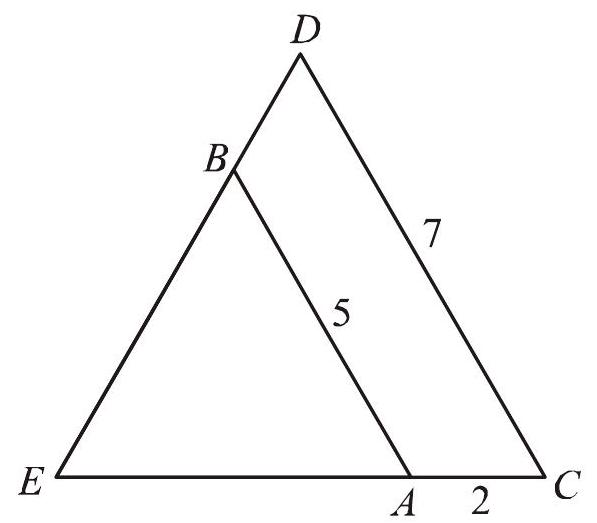
\includegraphics[max width=\textwidth, center]{2024_11_21_dcf819de2d2eef051a0dg-06(1)}

\section*{Zadanie 15. (1 pkt)}
Pole kwadratu wpisanego w okragg o promieniu 5 jest równe\\
A. 25\\
B. 50\\
C. 75\\
D. 100

\section*{Zadanie 16. (1 pkt)}
Punkty \(A, B, C, D\) dzielą okrąg na 4 równe fuki. Miara zaznaczonego na rysunku kąta wpisanego \(A C D\) jest równa\\
A. \(90^{\circ}\)\\
B. \(60^{\circ}\)\\
C. \(45^{\circ}\)\\
D. \(30^{\circ}\)\\
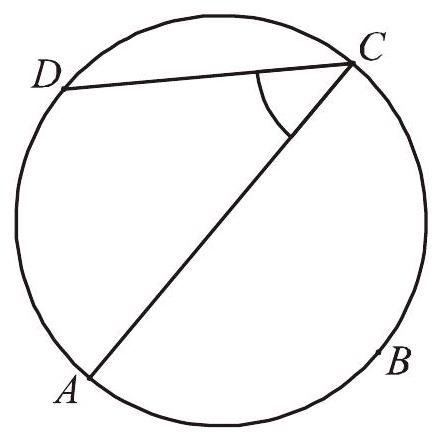
\includegraphics[max width=\textwidth, center]{2024_11_21_dcf819de2d2eef051a0dg-06}

\section*{Zadanie 17. (1 pkt)}
Miary kątów czworokąta tworzą ciąg arytmetyczny o różnicy \(20^{\circ}\). Najmniejszy kąt tego czworokąta ma miarę\\
A. \(40^{\circ}\)\\
B. \(50^{\circ}\)\\
C. \(60^{\circ}\)\\
D. \(70^{\circ}\)

\section*{Zadanie 18. (1 pkt)}
Dany jest ciag \(\left(a_{n}\right)\) określony wzorem \(a_{n}=(-1)^{n} \cdot \frac{2-n}{n^{2}}\) dla \(n \geq 1\). Wówczas wyraz \(a_{5}\) tego ciagu jest równy\\
A. \(-\frac{3}{25}\)\\
B. \(\frac{3}{25}\)\\
C. \(-\frac{7}{25}\)\\
D. \(\frac{7}{25}\)

\section*{BRUDNOPIS}
\begin{center}
\begin{tabular}{|c|c|c|c|c|c|c|c|c|c|c|c|c|c|c|c|c|c|c|c|c|c|c|c|}
\hline
 &  &  &  &  &  &  &  &  &  &  &  &  &  &  &  &  &  &  &  &  &  &  &  \\
\hline
 &  &  &  &  &  &  &  &  &  &  &  &  &  &  &  &  &  &  &  &  &  &  &  \\
\hline
 &  &  &  &  &  &  &  &  &  &  &  &  &  &  &  &  &  &  &  &  &  &  &  \\
\hline
 &  &  &  &  &  &  &  &  &  &  &  &  &  &  &  &  &  &  &  &  &  &  &  \\
\hline
 &  &  &  &  &  &  &  &  &  &  &  &  &  &  &  &  &  &  &  &  &  &  &  \\
\hline
 &  &  &  &  &  &  &  &  &  &  &  &  &  &  &  &  &  &  &  &  &  &  &  \\
\hline
 &  &  &  &  &  &  &  &  &  &  &  &  &  &  &  &  &  &  &  &  &  &  &  \\
\hline
 &  &  &  &  &  &  &  &  &  &  &  &  &  &  &  &  &  &  &  &  &  &  &  \\
\hline
 &  &  &  &  &  &  &  &  &  &  &  &  &  &  &  &  &  &  &  &  &  &  &  \\
\hline
 &  &  &  &  &  &  &  &  &  &  &  &  &  &  &  &  &  &  &  &  &  &  &  \\
\hline
 &  &  &  &  &  &  &  &  &  &  &  &  &  &  &  &  &  &  &  &  &  &  &  \\
\hline
 &  &  &  &  &  &  &  &  &  &  &  &  &  &  &  &  &  &  &  &  &  &  &  \\
\hline
 &  &  &  &  &  &  &  &  &  &  &  &  &  &  &  &  &  &  &  &  &  &  &  \\
\hline
 &  &  &  &  &  &  &  &  &  &  &  &  &  &  &  &  &  &  &  &  &  &  &  \\
\hline
 &  &  &  &  &  &  &  &  &  &  &  &  &  &  &  &  &  &  &  &  &  &  &  \\
\hline
 &  &  &  &  &  &  &  &  &  &  &  &  &  &  &  &  &  &  &  &  &  &  &  \\
\hline
 &  &  &  &  &  &  &  &  &  &  &  &  &  &  &  &  &  &  &  &  &  &  &  \\
\hline
 &  &  &  &  &  &  &  &  &  &  &  &  &  &  &  &  &  &  &  &  &  &  &  \\
\hline
 &  &  &  &  &  &  &  &  &  &  &  &  &  &  &  &  &  &  &  &  &  &  &  \\
\hline
 &  &  &  &  &  &  &  &  &  &  &  &  &  &  &  &  &  &  &  &  &  &  &  \\
\hline
 &  &  &  &  &  &  &  &  &  &  &  &  &  &  &  &  &  &  &  &  &  &  &  \\
\hline
 &  &  &  &  &  &  &  &  &  &  &  &  &  &  &  &  &  &  &  &  &  &  &  \\
\hline
 &  &  &  &  &  &  &  &  &  &  &  &  &  &  &  &  &  &  &  &  &  &  &  \\
\hline
 &  &  &  &  &  &  &  &  &  &  &  &  &  &  &  &  &  &  &  &  &  &  &  \\
\hline
 &  &  &  &  &  &  &  &  &  &  &  &  &  &  &  &  &  &  &  &  &  &  &  \\
\hline
 &  &  &  &  &  &  &  &  &  &  &  &  &  &  &  &  &  &  &  &  &  &  &  \\
\hline
 &  &  &  &  &  &  &  &  &  &  &  &  &  &  &  &  &  &  &  &  &  &  &  \\
\hline
 &  &  &  &  &  &  &  &  &  &  &  &  &  &  &  &  &  &  &  &  &  &  &  \\
\hline
 &  &  &  &  &  &  &  &  &  &  &  &  &  &  &  &  &  &  &  &  &  &  &  \\
\hline
 &  &  &  &  &  &  &  &  &  &  &  &  &  &  &  &  &  &  &  &  &  &  &  \\
\hline
 &  &  &  &  &  &  &  &  &  &  &  &  &  &  &  &  &  &  &  &  &  &  &  \\
\hline
 &  &  &  &  &  &  &  &  &  &  &  &  &  &  &  &  &  &  &  &  &  &  &  \\
\hline
 &  &  &  &  &  &  &  &  &  &  &  &  &  &  &  &  &  &  &  &  &  &  &  \\
\hline
 &  &  &  &  &  &  &  &  &  &  &  &  &  &  &  &  &  &  &  &  &  &  &  \\
\hline
 &  &  &  &  &  &  &  &  &  &  &  &  &  &  &  &  &  &  &  &  &  &  &  \\
\hline
 &  &  &  &  &  &  &  &  &  &  &  &  &  &  &  &  &  &  &  &  &  &  &  \\
\hline
 &  &  &  &  &  &  &  &  &  &  &  &  &  &  &  &  &  &  &  &  &  &  &  \\
\hline
 &  &  &  &  &  &  &  &  &  &  &  &  &  &  &  &  &  &  &  &  &  &  &  \\
\hline
 &  &  &  &  &  &  &  &  &  &  &  &  &  &  &  &  &  &  &  &  &  &  &  \\
\hline
 &  &  &  &  &  &  &  &  &  &  &  &  &  &  &  &  &  &  &  &  &  &  &  \\
\hline
 &  &  &  &  &  &  &  &  &  &  &  &  &  &  &  &  &  &  &  &  &  &  &  \\
\hline
 &  &  &  &  &  &  &  &  &  &  &  &  &  &  &  &  &  &  &  &  &  &  &  \\
\hline
 &  &  &  &  &  &  &  &  &  &  &  &  &  &  &  &  &  &  &  &  &  &  &  \\
\hline
 &  &  &  &  &  &  &  &  &  &  &  &  &  &  &  &  &  &  &  &  &  &  &  \\
\hline
 &  &  &  &  &  &  &  &  &  &  &  &  &  &  &  &  &  &  &  &  &  &  &  \\
\hline
 &  &  &  &  &  &  &  &  &  &  &  &  &  &  &  &  &  &  &  &  &  &  &  \\
\hline
 &  &  &  &  &  &  &  &  &  &  &  &  &  &  &  &  &  &  &  &  &  &  &  \\
\hline
 &  &  &  &  &  &  &  &  &  &  &  &  &  &  &  &  &  &  &  &  &  &  &  \\
\hline
 &  &  &  &  &  &  &  &  &  &  &  &  &  &  &  &  &  &  &  &  &  &  &  \\
\hline
\end{tabular}
\end{center}

\section*{Zadanie 19. (1 pkt)}
Pole powierzchni jednej ściany sześcianu jest równe 4. Objętość tego sześcianu jest równa\\
A. 6\\
B. 8\\
C. 24\\
D. 64

\section*{Zadanie 20. (1 pkt)}
Tworząca stożka ma długość 4 i jest nachylona do płaszczyzny podstawy pod kątem \(45^{\circ}\). Wysokość tego stożka jest równa\\
A. \(2 \sqrt{2}\)\\
B. \(16 \pi\)\\
C. \(4 \sqrt{2}\)\\
D. \(8 \pi\)

\section*{Zadanie 21. (1 pkt)}
Wskaż równanie prostej równoległej do prostej o równaniu \(3 x-6 y+7=0\).\\
A. \(y=\frac{1}{2} x\)\\
B. \(y=-\frac{1}{2} x\)\\
C. \(y=2 x\)\\
D. \(y=-2 x\)

\section*{Zadanie 22. (1 pkt)}
Punkt \(A\) ma współrzędne \((5,2012)\). Punkt \(B\) jest symetryczny do punktu \(A\) względem osi \(O x\), a punkt \(C\) jest symetryczny do punktu \(B\) względem osi \(O y\). Punkt \(C\) ma wspórzzędne\\
A. \((-5,-2012)\)\\
B. \((-2012,-5)\)\\
C. \((-5,2012)\)\\
D. \((-2012,5)\)

\section*{Zadanie 23. (1 pkt)}
Na okręgu o równaniu \((x-2)^{2}+(y+7)^{2}=4\) leży punkt\\
A. \(A=(-2,5)\)\\
B. \(B=(2,-5)\)\\
C. \(\quad C=(2,-7)\)\\
D. \(D=(7,-2)\)

\section*{Zadanie 24. (1 pkt)}
Flage, taką jak pokazano na rysunku, należy zszyć z trzech jednakowej szerokości pasów kolorowej tkaniny. Oba pasy zewnętrzne mają być tego samego koloru, a pas znajdujący się między nimi ma być innego koloru.\\
Liczba różnych takich flag, które można uszyć, mając do dyspozycji tkaniny w 10 kolorach, jest równa\\
A. 100\\
B. 99\\
C. 90\\
D. 19

\section*{Zadanie 25. (1 pkt)}
Średnia arytmetyczna cen sześciu akcji na giełdzie jest równa 500 zk . Za pięć z tych akcji zapłacono 2300 zł. Cena szóstej akcji jest równa\\
A. \(400 \mathrm{zł}\)\\
B. 500 zt\\
C. 600 zt\\
D. 700 zk

\section*{BRUDNOPIS}
\begin{center}

\includegraphics[max width=\textwidth]{2024_11_21_dcf819de2d2eef051a0dg-09}
\end{center}

\section*{ZADANIA OTWARTE}
\section*{Rozwiqzania zadań o numerach od 26. do 34. nalė̇y zapisać w wyznaczonych miejscach pod treściq zadania.}
\section*{Zadanie 26. (2 pkt)}
Rozwiąż nierówność \(x^{2}+8 x+15>0\).\\

\includegraphics[max width=\textwidth, center]{2024_11_21_dcf819de2d2eef051a0dg-10}

Odpowiedź:

\section*{Zadanie 27. (2 pkt)}
Uzasadnij, że jeśli liczby rzeczywiste \(a, b, c\) spełniają nierówności \(0<a<b<c\), to \(\frac{a+b+c}{3}>\frac{a+b}{2}\).\\

\includegraphics[max width=\textwidth, center]{2024_11_21_dcf819de2d2eef051a0dg-10(1)}

\section*{Zadanie 28. (2 pkt)}
Liczby \(x_{1}=-4\) i \(\quad x_{2}=3\) są pierwiastkami wielomianu \(W(x)=x^{3}+4 x^{2}-9 x-36\). Oblicz trzeci pierwiastek tego wielomianu.\\

\includegraphics[max width=\textwidth, center]{2024_11_21_dcf819de2d2eef051a0dg-11}

Odpowiedź:

\section*{Zadanie 29. (2 pkt)}
Wyznacz równanie symetralnej odcinka o końcach \(A=(-2,2)\) i \(B=(2,10)\).\\

\includegraphics[max width=\textwidth, center]{2024_11_21_dcf819de2d2eef051a0dg-11(1)}

Odpowiedź:

\begin{center}
\begin{tabular}{|c|l|c|c|c|c|}
\hline
\multirow{2}{*}{\begin{tabular}{c}
Wypełnia \\
egzaminator \\
\end{tabular}} & Nr zadania & 26. & 27. & 28. & 29. \\
\cline { 2 - 6 }
 & Maks. liczba pkt & 2 & 2 & 2 & 2 \\
\cline { 2 - 6 }
 & Uzyskana liczba pkt &  &  &  &  \\
\hline
\end{tabular}
\end{center}

Zadanie 30. (2 pkt)\\
W trójkaçie \(A B C\) poprowadzono dwusieczne katów \(A\) i \(B\). Dwusieczne te przecinają się w punkcie \(P\). Uzasadnij, że kąt \(A P B\) jest rozwarty.

\begin{center}
\begin{tabular}{|c|c|c|c|c|c|c|c|c|c|c|c|c|c|c|c|c|c|c|c|c|c|c|}
\hline
 &  &  &  &  &  &  &  &  &  &  &  &  &  &  &  &  &  &  &  &  &  &  \\
\hline
 &  &  &  &  &  &  &  &  &  &  &  &  &  &  &  &  &  &  &  &  &  &  \\
\hline
 &  &  &  &  &  &  &  &  &  &  &  &  &  &  &  &  &  &  &  &  &  &  \\
\hline
 &  &  &  &  &  &  &  &  &  &  &  &  &  &  &  &  &  &  &  &  &  &  \\
\hline
 &  &  &  &  &  &  &  &  &  &  &  &  &  &  &  &  &  &  &  &  &  &  \\
\hline
 &  &  &  &  &  &  &  &  &  &  &  &  &  &  &  &  &  &  &  &  &  &  \\
\hline
 &  &  &  &  &  &  &  &  &  &  &  &  &  &  &  &  &  &  &  &  &  &  \\
\hline
 &  &  &  &  &  &  &  &  &  &  &  &  &  &  &  &  &  &  &  &  &  &  \\
\hline
 &  &  &  &  &  &  &  &  &  &  &  &  &  &  &  &  &  &  &  &  &  &  \\
\hline
 &  &  &  &  &  &  &  &  &  &  &  &  &  &  &  &  &  &  &  &  &  &  \\
\hline
 &  &  &  &  &  &  &  &  &  &  &  &  &  &  &  &  &  &  &  &  &  &  \\
\hline
 &  &  &  &  &  &  &  &  &  &  &  &  &  &  &  &  &  &  &  &  &  &  \\
\hline
 &  &  &  &  &  &  &  &  &  &  &  &  &  &  &  &  &  &  &  &  &  &  \\
\hline
 &  &  &  &  &  &  &  &  &  &  &  &  &  &  &  &  &  &  &  &  &  &  \\
\hline
 &  &  &  &  &  &  &  &  &  &  &  &  &  &  &  &  &  &  &  &  &  &  \\
\hline
 &  &  &  &  &  &  &  &  &  &  &  &  &  &  &  &  &  &  &  &  &  &  \\
\hline
 &  &  &  &  &  &  &  &  &  &  &  &  &  &  &  &  &  &  &  &  &  &  \\
\hline
 &  &  &  &  &  &  &  &  &  &  &  &  &  &  &  &  &  &  &  &  &  &  \\
\hline
 &  &  &  &  &  &  &  &  &  &  &  &  &  &  &  &  &  &  &  &  &  &  \\
\hline
 &  &  &  &  &  &  &  &  &  &  &  &  &  &  &  &  &  &  &  &  &  &  \\
\hline
 &  &  &  &  &  &  &  &  &  &  &  &  &  &  &  &  &  &  &  &  &  &  \\
\hline
 &  &  &  &  &  &  &  &  &  &  &  &  &  &  &  &  &  &  &  &  &  &  \\
\hline
 &  &  &  &  &  &  &  &  &  &  &  &  &  &  &  &  &  &  &  &  &  &  \\
\hline
 &  &  &  &  &  &  &  &  &  &  &  &  &  &  &  &  &  &  &  &  &  &  \\
\hline
 &  &  &  &  &  &  &  &  &  &  &  &  &  &  &  &  &  &  &  &  &  &  \\
\hline
 &  &  &  &  &  &  &  &  &  &  &  &  &  &  &  &  &  &  &  &  &  &  \\
\hline
 &  &  &  &  &  &  &  &  &  &  &  &  &  &  &  &  &  &  &  &  &  &  \\
\hline
 &  &  &  &  &  &  &  &  &  &  &  &  &  &  &  &  &  &  &  &  &  &  \\
\hline
 &  &  &  &  &  &  &  &  &  &  &  &  &  &  &  &  &  &  &  &  &  &  \\
\hline
 &  &  &  &  &  &  &  &  &  &  &  &  &  &  &  &  &  &  &  &  &  &  \\
\hline
 &  &  &  &  &  &  &  &  &  &  &  &  &  &  &  &  &  &  &  &  &  &  \\
\hline
 &  &  &  &  &  &  &  &  &  &  &  &  &  &  &  &  &  &  &  &  &  &  \\
\hline
 &  &  &  &  &  &  &  &  &  &  &  &  &  &  &  &  &  &  &  &  &  &  \\
\hline
 &  &  &  &  &  &  &  &  &  &  &  &  &  &  &  &  &  &  &  &  &  &  \\
\hline
 &  &  &  &  &  &  &  &  &  &  &  &  &  &  &  &  &  &  &  &  &  &  \\
\hline
 &  &  &  &  &  &  &  &  &  &  &  &  &  &  &  &  &  &  &  &  &  &  \\
\hline
 &  &  &  &  &  &  &  &  &  &  &  &  &  &  &  &  &  &  &  &  &  &  \\
\hline
 &  &  &  &  &  &  &  &  &  &  &  &  &  &  &  &  &  &  &  &  &  &  \\
\hline
 &  &  &  &  &  &  &  &  &  &  &  &  &  &  &  &  &  &  &  &  &  &  \\
\hline
 &  &  &  &  &  &  &  &  &  &  &  &  &  &  &  &  &  &  &  &  &  &  \\
\hline
 &  &  &  &  &  &  &  &  &  &  &  &  &  &  &  &  &  &  &  &  &  &  \\
\hline
 &  &  &  &  &  &  &  &  &  &  &  &  &  &  &  &  &  &  &  &  &  &  \\
\hline
 &  &  &  &  &  &  &  &  &  &  &  &  &  &  &  &  &  &  &  &  &  &  \\
\hline
 &  &  &  &  &  &  &  &  &  &  &  &  &  &  &  &  &  &  &  &  &  &  \\
\hline
 &  &  &  &  &  &  &  &  &  &  &  &  &  &  &  &  &  &  &  &  &  &  \\
\hline
 &  &  &  &  &  &  &  &  &  &  &  &  &  &  &  &  &  &  &  &  &  &  \\
\hline
\end{tabular}
\end{center}

\section*{Zadanie 31. (2 pkt)}
Ze zbioru liczb \{1,2,3,4,5,6,7\} losujemy dwa razy po jednej liczbie ze zwracaniem. Oblicz prawdopodobieństwo zdarzenia \(A\), polegającego na wylosowaniu liczb, których iloczyn jest podzielny przez 6.\\

\includegraphics[max width=\textwidth, center]{2024_11_21_dcf819de2d2eef051a0dg-13}

Odpowiedź:

\begin{center}
\begin{tabular}{|c|l|c|c|}
\hline
\multirow{2}{*}{\begin{tabular}{c}
Wypetnia \\
egzaminator \\
\end{tabular}} & Nr zadania & 30. & 31. \\
\cline { 2 - 4 }
 & Maks. liczba pkt & \(\mathbf{2}\) & \(\mathbf{2}\) \\
\cline { 2 - 4 }
 & Uzyskana liczba pkt &  &  \\
\hline
\end{tabular}
\end{center}

\section*{Zadanie 32. (4 pkt)}
Ciag \((9, x, 19)\) jest arytmetyczny, a ciąg \((x, 42, y, z)\) jest geometryczny. Oblicz \(x, y\) oraz \(z\).\\

\includegraphics[max width=\textwidth, center]{2024_11_21_dcf819de2d2eef051a0dg-14}

\section*{Zadanie 33. (4 pkt)}
W graniastosłupie prawidłowym czworokątnym \(A B C D E F G H\) przekątna \(A C\) podstawy ma długość 4 . Kąt \(A C E\) jest równy \(60^{\circ}\). Oblicz objętość ostrosłupa \(A B C D E\) przedstawionego na poniższym rysunku.\\
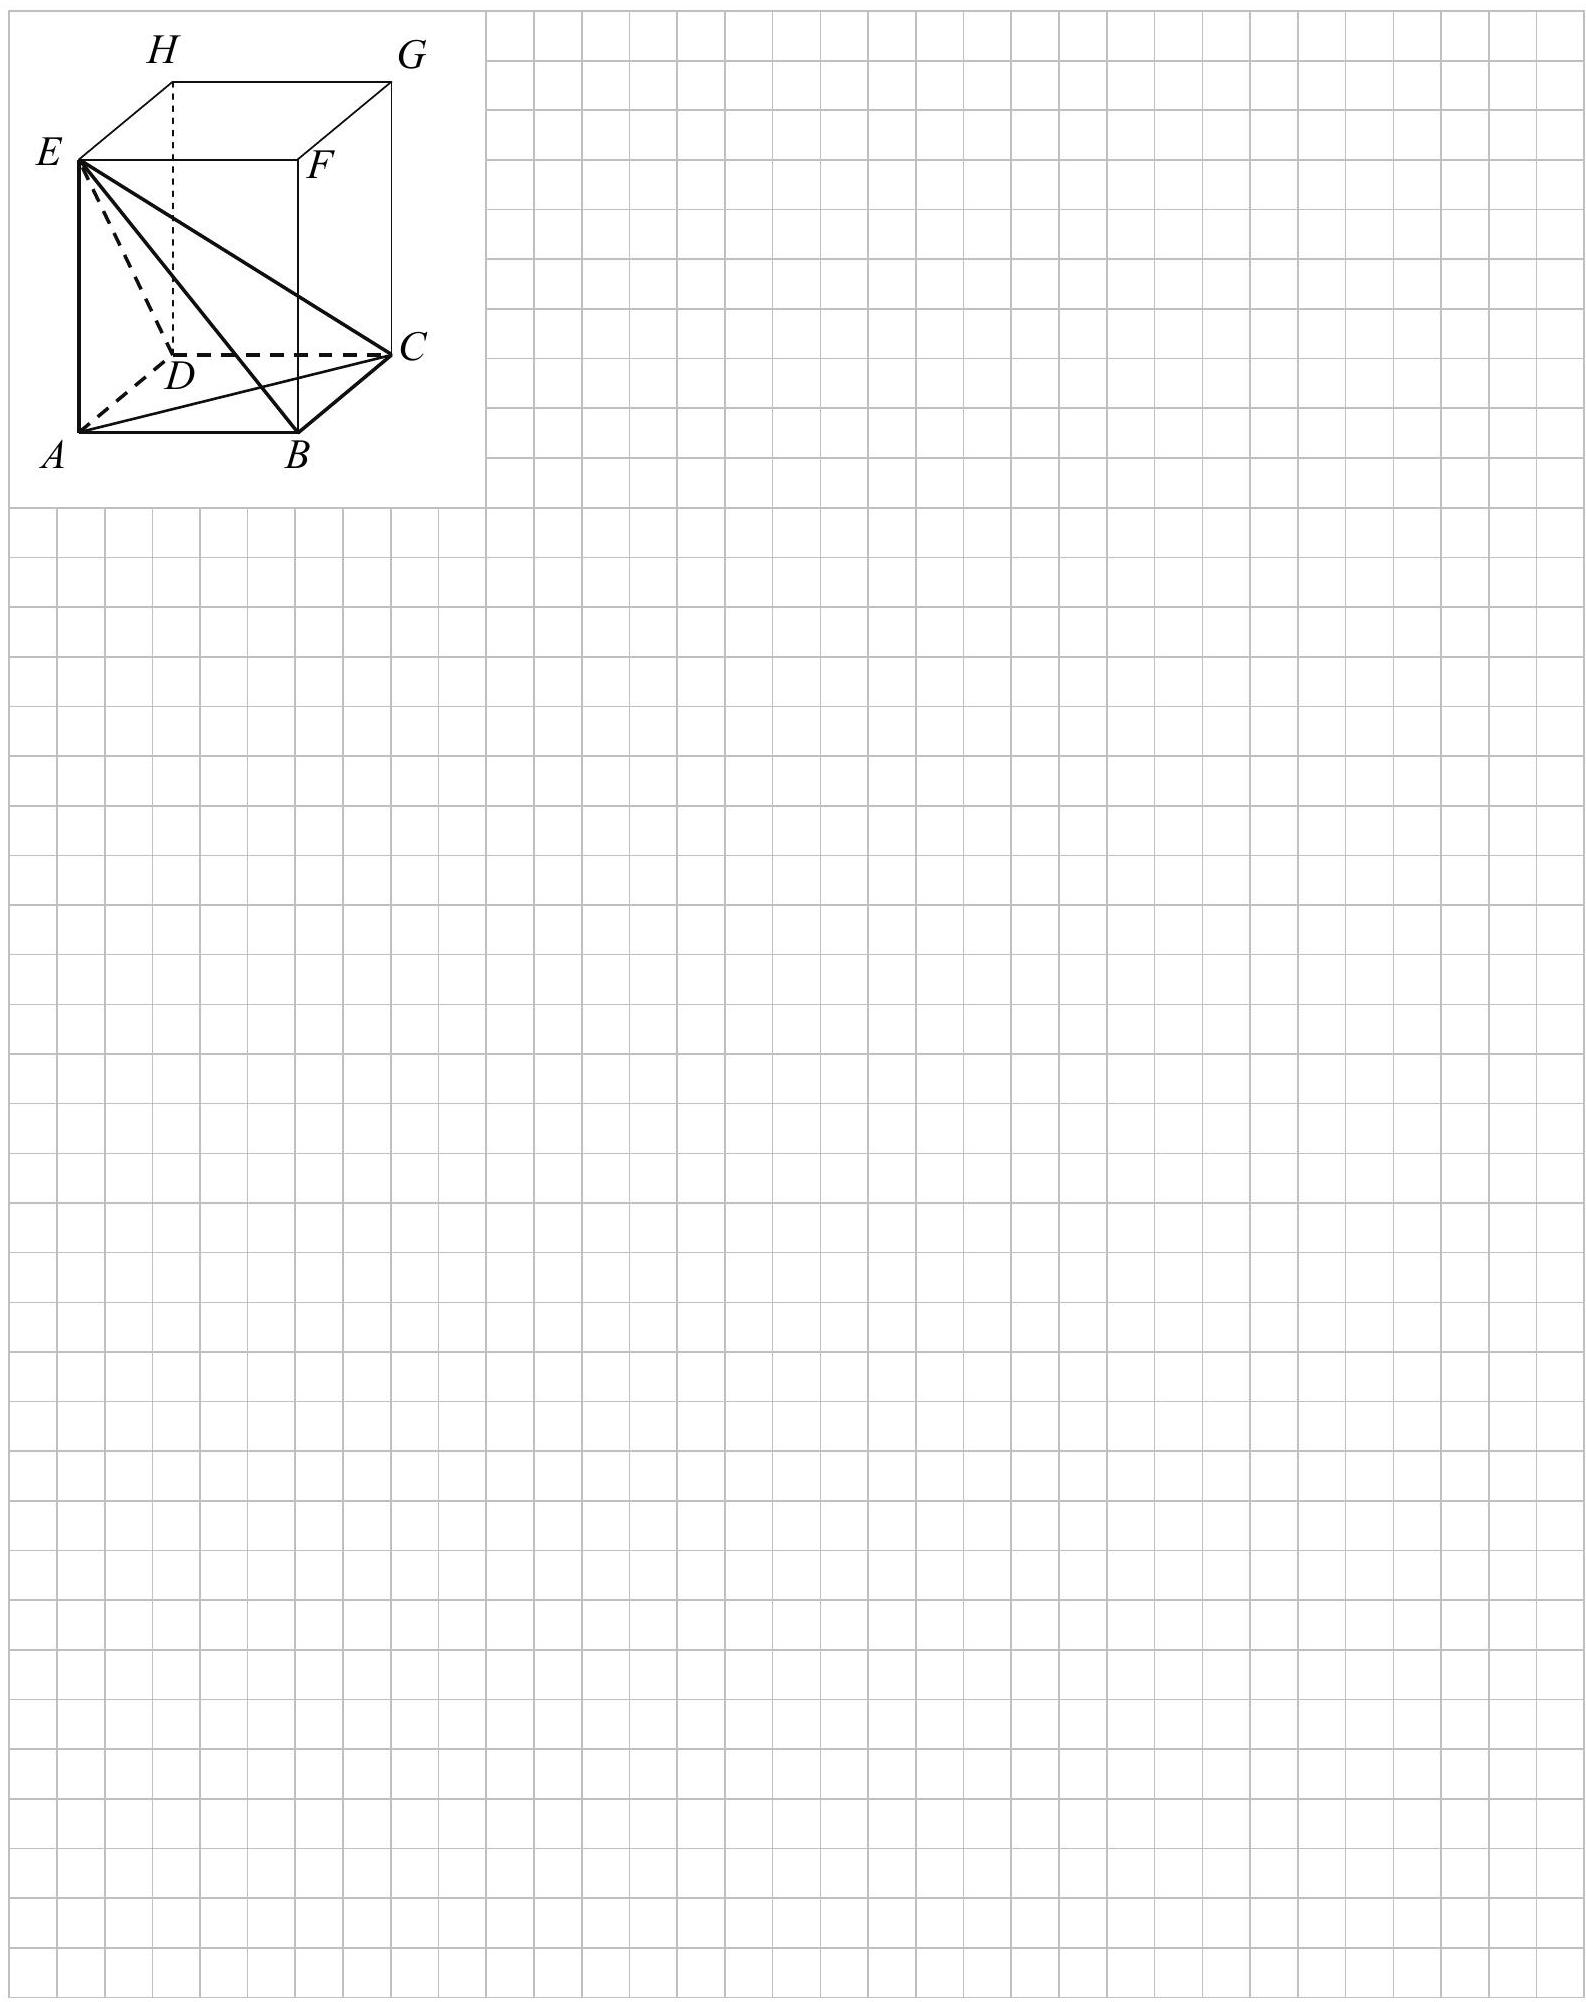
\includegraphics[max width=\textwidth, center]{2024_11_21_dcf819de2d2eef051a0dg-15}

Odpowiedź:

\begin{center}
\begin{tabular}{|c|l|c|c|}
\hline
\multirow{2}{*}{\begin{tabular}{c}
Wypetnia \\
egzaminator \\
\end{tabular}} & Nr zadania & 32. & 33. \\
\cline { 2 - 4 }
 & Maks. liczba pkt & 4 & 4 \\
\cline { 2 - 4 }
 & Uzyskana liczba pkt &  &  \\
\hline
\end{tabular}
\end{center}

\section*{Zadanie 34. (5 pkt)}
Miasto \(A\) i miasto \(B\) łaczy linia kolejowa długości 210 km . Średnia prędkość pociagu pospiesznego na tej trasie jest o \(24 \mathrm{~km} / \mathrm{h}\) większa od średniej prędkości pociagu osobowego. Pociagg pospieszny pokonuje tę trasę o 1 godzinę krócej niż pociag osobowy. Oblicz czas pokonania tej drogi przez pociag pospieszny.\\

\includegraphics[max width=\textwidth, center]{2024_11_21_dcf819de2d2eef051a0dg-16}\\

\includegraphics[max width=\textwidth, center]{2024_11_21_dcf819de2d2eef051a0dg-17}

Odpowiedź:

\begin{center}
\begin{tabular}{|c|l|c|}
\hline
\multirow{2}{*}{\begin{tabular}{l}
Wypelnia \\
egzaminator \\
\end{tabular}} & Nr zadania & 34. \\
\cline { 2 - 3 }
 & Maks. liczba pkt & 5 \\
\cline { 2 - 3 }
 & Uzyskana liczba pkt &  \\
\hline
\end{tabular}
\end{center}

\section*{BRUDNOPIS}

\end{document}